\documentclass[11pt]{article}  
\usepackage[margin=1in]{geometry}
\usepackage{authblk}
\usepackage{graphicx}
\usepackage[fleqn]{amsmath}

%\usepackage{ltexpprt} 

\begin{document}
\title{\Large Joint Optimization of Routing and Node Selection}
%\thanks{Supported by .} 
\author[]{Moses Charikar}
\author[]{Yonatan Naamad}
\author[]{Jennifer Rexford}
\author[]{X. Kelvin Zou}
\affil[]{Department of Computer Science, Princeton University}
\affil[ ]{\textit {\{moses,ynaamad,jrex, xuanz\}@cs.princeton.edu}}
\date{}
\maketitle

\section{Introduction}

\subsection{The basic problem}
Networks have evolved beyond a simple packet forwarding. Many types of in-network flow processing are ubiquitous today. The flow processing usually take place at vertices, in which we install one or a few appliances, so called middleboxes(MBoxes), examples including firewall and network proxy. Having the flow going through MBox(es) for processing enriches the network functions and policies. The placement of MBoxes is an essential component in network design problem. Today some network designs choose to treat the MBoxes as an overlay on top of the routing: the designs abstract the connection between the source and the MBox, the MBox and the sink as virtually directly connected edges, and the "virtual connection" is handled underneath by routing\cite{SIMPLE2013}. The abstraction bypasses the problem but leads to inefficient routing and bouncing traffic. Other designs utilize special network topologies such as FatTree\cite{FATTREE} in the data centers and place at choke points, but it fails to cover generalized cases and is hard to balance the load across the MBoxes. 

In this paper we extract the problem of the MBox placement as a graph model. The flow's in-network processing can be divided into multiple parts and take place in distributed vertices, and collectively all the contributing vertices handle the whole flow.  As each flow requires a certain amount of in-network processing, sending a flow from a source to a sink is not only constrained by the edge capacity; it is also limited by the processing capacity of vertices. The in-network processing required for a flow is proportional to the flow size. Without losing generality, we assume the ratio is 1, that is one unit of flow requires one unit of processing. 

To capture both the capacitated vertices and edges, we state the graph model as the following:
a directed graph $G(V,E)$ where each edge $e\in E$ has an edge bandwidth $B(e)$, and each vertex $v\in V$ has a processing capacity $C(v)$. 
We define a feasible flow from a source to a sink on a path $p$ such that it has to satisfy both the edge and vertex constraints: the flow size $f $ cannot violate any edge $e$'s capacity on the path, i.e., $f\leq B(e)$ for $\forall e\in p$; and the collection of vertices $v$ where $v\in p$ can handle $f$, i.e., $f\leq\sum\limits_{v\in p}C(v)$. 
\begin{figure}[h]
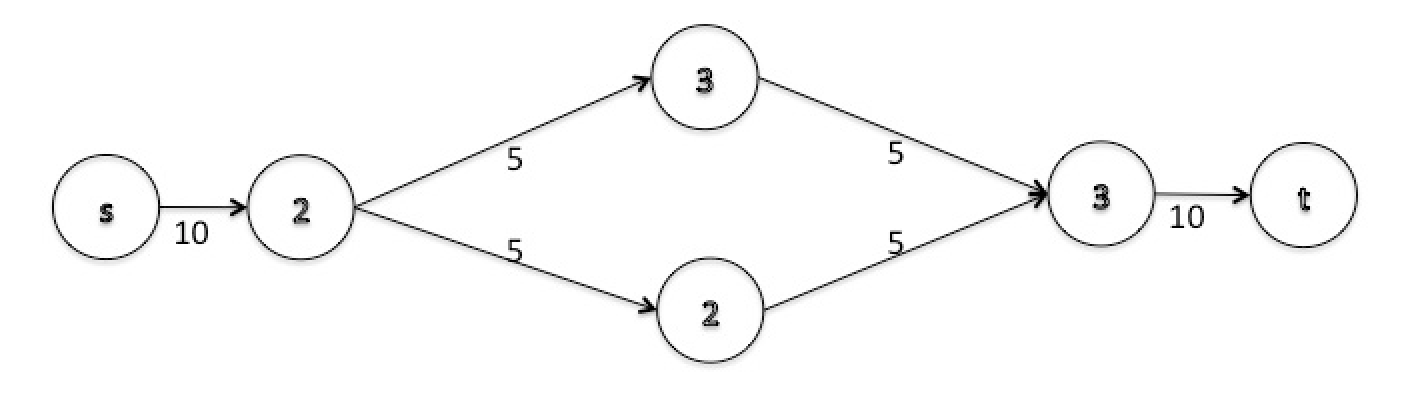
\includegraphics[width=\linewidth]{picture1.png} 
\caption{ \textbf{Example for the Graph Model: given the edge and vertex constraints, \textnormal{\{5,10\} }are edge capacities and \{2,3\} are vertex capacities, the maximum flow from source to sink in the example is 10, in this example all edges and vertices will be saturated.} }
 \end{figure}
 
Network design problems involve finding a network with a minimum cost that satisfies various properties, often related to routing and flow feasibility. The network design problem in this model is: for a multi-source and multi-sink flow demand, and a fixed amount of budget for the processing capacities, or MBoxes among the vertices, what is the optimal way of placing them? This network design problem answers optimal placement of MBoxes for a given network with a certain flow pattern. 

This problem covers a superset of multi-commodity flow problem\cite{MCF}, that is, if we can solve this problem, we can naturally solve multi-commodity flow problem: simply assign each vertex with an infinite capacity it becomes an MCF problem. Many classic MCF problems can be extended to this superset, such as MC-BB(multi-commodity buy-at-bulk) problem\cite{BuyAtBulk,Charikar05,Chekuri2007}. 

\subsection{The results in this paper}



\section{Processing Capacity Placement in fractional manner}
We formulate a generalized linear programming model in this problem in an edge based formulation. Notations: $C(v),B(e)$ represents the processing and edge capacity at node $v$ and edge $e$, $f_i(e)$ represents the flow size for each source-sink pair on edge $e$, $w_i(e)$ represents process demand for flow i carried out at edge $e$, $f(C(v))$ is an concave cost function of $C(v)$: 

\begin{equation*}
\begin{aligned}
\text{Minimize:}&\sum\limits_v f(C(v))\\
\text{Subject to:}&\\
&\forall v \in V-\{s, t\}, \forall i, \sum\limits_{in}  f_i(e)=  \sum\limits_{out} f_i(e);\\
&\forall e, \sum\limits_{i} f_{i}(e)\leq B(e);\\
&\forall e,\forall  i,0 \leq w_i(e) \leq f_i(e),\\
&\forall v,\forall  i, 0\leq \sum\limits_{in } w_i(e) - \sum\limits_{out} w_i(e)   \leq{C(v)}.\\
%&\forall i, \sum\limits_v f_i(s, v) = r_i; \\
&\forall  i; \forall (s, v), w_i = f_i\;\&\; \forall (v,t), w_i =0.
\end{aligned}
\end{equation*}




\bibliographystyle{acm}
\bibliography{references}

\appendix
\end{document}